\chapter{Predictive Models}

The most common framework in ML is to construct \textbf{predictive models} capable of making predictions by looking at a set of data which may be uncertain, noisy, or incomplete. Predictive models are also useful when the theory behind a certain phenomenon is poor or completely absent. ML studies and proposes methods to infer \textbf{functions} from \textbf{examples} of observed data. Such function must:
    \begin{itemize}
        \item \textbf{fit} the example data;
        \item \textbf{generalize} with reasonable accuracy.
    \end{itemize}

A simple example might be recognizing handwritten numbers. The model is presented with some real-life data (pictures of numbers written on paper), and then approximates a function capable of recognizing numbers out of pictures never seen before. 

\section{Components of a Model}

A predictive system can be broken down into the following key components:

\begin{itemize}
    \item Data;
    \item Task;
    \item Model;
    \item Learning algorithm;
    \item Validation;
    \item Prediction.
\end{itemize}

\subsection{Data}

The data represents the available facts. Can be either flat (attribute-value language, fixed-size vector), or structured (more complex data structures).

\textbf{Flat data} can be represented as a table with multiple rows and columns.

\begin{itemize}
    \item Rows: \textbf{examples}, patterns, instances, samples...
    \item Columns: \textbf{features}, attributes, elements, components...
    \item The number of examples is the dimension of the dataset;
    \item The number of features per example is the dimension of the input;
    \item Examples and attributes can be indexed: e.g., $x_i$ is the $i^{th}$ feature of element $x$; \bm$x_i$ is the $i^{th}$ element; $x_{p,i}$ is the $i^{th}$ feature of the $p^{th}$ example.
\end{itemize}

It is often useful to \textbf{encode} the data. Structured data is a complex data structure, such as a list, tree, graph, multi-relational data, etc.

\BoxDef{Noise}{
Noise is the addition of external factors to the stream of information caused by randomness in measurements (which are never always 100\% accurate)
}

\BoxDef{Outliers}{
Outliers are unusual data values, inconsistent with most observations (may be caused by incorrect measurements). They can be removed by appropriate preprocessing (outlier detection).
}

\BoxDef{Feature selection}{
The selection of a subset of features deemed informative. Can provide an optimal input representation for the data.
}

\subsection{Task}

The task defines the purpose of the application: what information do we want to achieve? What can the result be used for? What data is available?

\BoxDef{Supervised Learning}{
\begin{itemize}
    \item \textbf{Given}: a \textbf{training set (TR)} consisting of training examples \bm{$<input,output>$} = \bm{$<x,d>$} (where $d$ is the \textbf{target value}, a categorical or numerical \textbf{label}) for an unknown function \bm{$f$} (called \textbf{target function}).
    
    \item \textbf{Find}: a "good" approximation of $f$, called \textbf{hypothesis} \bm{$h$}, that can be used on unseen data to predict its value according to $f$ (= is able to \textbf{generalize}).
\end{itemize}
}

\textbf{Unsupervised learning} is defined the same as the above, but the input data is a TR of unlabeled data.


\BoxDef{Types of tasks}{
\begin{itemize}
    \item \textbf{Classification}: input vectors are seen as members of two or more classes; the goal is to assign a class to any input $x$. The function produces discrete valued outputs (corresponding to the different classes found).

    If the number of classes is 2, the task is binary classification. Otherwise, it's a multi-class problem.

    \item \textbf{Regression}: estimate a real-value function on the basis of a finite set of (noisy) examples.

    \item *and more*
\end{itemize}
}

\subsection{Model}

A model describes the relationships among the data by using a "language" (numerical, symbolic,...). The model also defines the set of function the learning machine can implement: the \textbf{hypotheses space H}. 

Many models exist as of today: linear models, symbolic rules, probabilistic models, etc. Why so many? Because \href{https://en.wikipedia.org/wiki/No_free_lunch_theorem}{\textit{there is no free lunch}}: each model is effective and efficient for some problems and not others, has different levels of flexibility, and has different ways to control its complexity.

\subsection{Learning Algorithm}

Given data, task, and model, the learning algorithm executes an \textbf{heuristic search} in the hypotheses space H, in order to find the "best" hypothesis that approximates the target function. By "best", we mean the function with the \textbf{minimum error}.

In order to setup a model, we must make assumptions about the target function, regarding either/both:

\begin{itemize}
    \item Constraints in the model: \textbf{language bias};
    \item Constraints in the learning algorithm: \textbf{search bias}.
\end{itemize}

To explain why such biases are needed, an example is presented.
We want to approximate a boolean function $f$, and we are given a certain number of examples, each of $n$ features, and paired to a label (the output, 0/1).

If we want to search for the best approximation of $f$, we would have to search throughout all the boolean functions in the hypotheses space H; the dimension of H is $2^{2^n}$ ($2$ = number of possible outputs, $2^n$ = number of possible inputs). Even if we found a function that matched the examples, it would be essentially \textbf{incapable of generalizing}: if the learner receives an input it already saw, it can classify it, otherwise it can't produce an output (it's essentially a lookup table). 

\begin{center}
    \vspace{5mm}
    \boxed{\textbf{NO INDUCTIVE BIAS $\xrightarrow{}$ NO GENERALIZATION}}
    \vspace{5mm}
\end{center}

We can introduce a language bias to limit the number of hypotheses to search through.
For example: let us use conjunctive rules to express the hypotheses (functions can only be propositions connected by the AND operator). The number of total functions that can be expressed in this notation lowers to $3^n + 1$ (total of $n$ possible literals per rule, each literal can be either true, false, or not appear at all; the extra 1 is the hypothesis that always evaluates to false).

\BoxDef{Consistency and version space}{
An hypothesis $h$ is \textbf{consistent} with a training set TR if $h(x)=d$ for each training example $<x,d>$ in TR. The set of all hypotheses in H consistent with a TR is called \textbf{version space (VS)} (can also be referred to as \bm{$VS_{H,TR}$}).
}

Many algorithms exist that can perform a complete search in the hypotheses space H, as in, that are capable of identifying the version space with respect to a TR. However, when using language biases, the restriction of the hypotheses space may be excessive, with the risk of excluding the target function: e.g., referring to the previous example, any rule that uses disjunction (OR operator) would be excluded from the search altogether.

The other approach is to instead use a language capable of expressing all possible hypotheses, and introduce a search bias, using an incomplete search strategy. 

\BoxDef{Loss and error}{
In order to measure the "goodness" of an hypothesis $h$, an inner measure is used, called the \textbf{loss function (or loss measure)}: \bm{$L(h(x),d)$}. The expected value of $L$ is called the \text{error} relative to $h$.
}

The loss function and the error can be calculated in any different ways depending on tasks. The following list presents some commonly used loss and error functions ("$w$" in the error function refers to the vector of parameters that identify that specific $h$).

\begin{itemize}
    \item \textbf{Regression}: predicting a numerical value.
    
    \textbf{H}: set of real-valued funcs.
    
    \textbf{L}: $L(h(x_p),d_p) = (d_p - h(x_p))^2$ (squared error)
    
    \textbf{E}: $E(h_w) = \dfrac{1}{l} \sum_{p=1}^l (d_p - h_w(x_p))^2$ (mean squared error)

    \item \textbf{Classification}: classifying data into two or more classes.

    \textbf{H}: a set of indicator functions (discrete-valued).
    
    \textbf{L}: $L(h(x_p),d_p) = \begin{cases}
                                    0 & \text{if } h(x_p) = d_p \\
                                    1 & \text{otherwise}
                                \end{cases}$
                                    
    \textbf{E}: $E(h_w) = $ mean over the data set providing \% of misclassified patterns

    \item \textbf{Clustering}: partitioning data in clusters, each approximated by a centroid/ prototype.

    \textbf{H}: set of vector quantizers.
    
    \textbf{L}: $L(h(x_p), d_p) = (x_p - h(x_p)) * (x_p - h(x_p))$ (squared error distortion)

    \textbf{E}: TBD

    \item \textbf{Density estimation}: estimating density from an assumed class.

    \textbf{H}: set of density funcs.

    \textbf{L}: $L(h(x_p), d_p) = -\ln{h(x_p)}$

    \textbf{E}: TBD
\end{itemize}

Error is calculated by measuring loss on new samples of data (a set of labeled examples).

\subsection{Validation}

Validation is the evaluation of performances in ML systems. Any $h$ that approximates the target function $f$ correctly on training examples should also approximate $f$ well on unseen examples.

\BoxDef{Overfitting}{
A learner \textbf{overfits} the data if it outputs an hypothesis $h \in H$ with true/generalization error $R$ and empirical (training) error $E$, but there's a $h' \in H$ with error $R' < R$ and $E' > E$.
}

\begin{center}
    \vspace{5mm}
    \boxed{\textbf{OVERFITTING \underline{DOES NOT} DEPEND ON NOISE}}
    \vspace{5mm}
\end{center}

Overfitting is caused by choosing a model with a complexity such that it adapts too much to the data (noisy data as well), but the presence of noise does not automatically equate to an overfit model.

\BoxDef{Underfitting}{
A learner \textbf{underfits} the data if it outputs an hypothesis with both very high values of generalization error $R$ and empirical error $E$; i.e., the model is too simple to accurately approximate the target function.
}

\section{Statistical Learning Theory}

Statistical Learning Theory (SLT) studies the properties of models to determine their generalization capability, with respect to the training error and underfitting/overfitting zones.

\subsection{VC-bound}

To approximate a target function $f$, the learner must find the hypothesis $h$ with the minimum \textbf{risk function}: \bm{$R = \int L(d, h(x)) dP(x,d)$}, where $P(x,d)$ is a probability distribution. However, when constructing a model, we can only calculate what is the value of the \textbf{empirical risk} \bm{$R_{emp}$} (also called training error E). We can use it to approximate $R$ by indicating an upper bound for it.

Given the \textbf{VC-dim / VC} (Vapnik-Chervonenkis-dim), a measure of the complexity of $H$, then it holds with probability $1-\delta$ the following inequality:

\begin{center}
    \bm{$R \leq R_{emp} + \epsilon(1/l, VC, 1/\delta)$}
\end{center}

Function $\epsilon$ is called \textbf{VC-confidence} and is defined so that it is directly proportional to $VC$, and inversely proportional to $l$ (the dimension of the TR) and $\delta$ (the chosen confidence). With this bound, we can explain undefitting and overfitting in a more formal way:

\begin{itemize}
    \item \textbf{If l is big}: value of $\epsilon$ is low, bound mostly depends of $R_{emp}$ $\xrightarrow{}$ \textbf{enough data to approximate target function};

    \item \textbf{If l is low}: value of $\epsilon$ is high causing the upper bound to increase, regardless of $R_{emp}$ $\xrightarrow{}$ \textbf{too little data to approximate target function};

    \item \textbf{If VC-dim is high}: $R_{emp}$ is low but $\epsilon$ is high, model may be too complex $\xrightarrow{}$ \textbf{overfitting};

    \item \textbf{If VC-dim is low}: $\epsilon$ is low but $R_{emp}$ is high, model may be too simple $\xrightarrow{}$ \textbf{underfitting}.
\end{itemize}

The goal now is to minimize this bound by finding the best trade-off between model complexity and fitting of training data.

\begin{figure}[h]
    \centering
    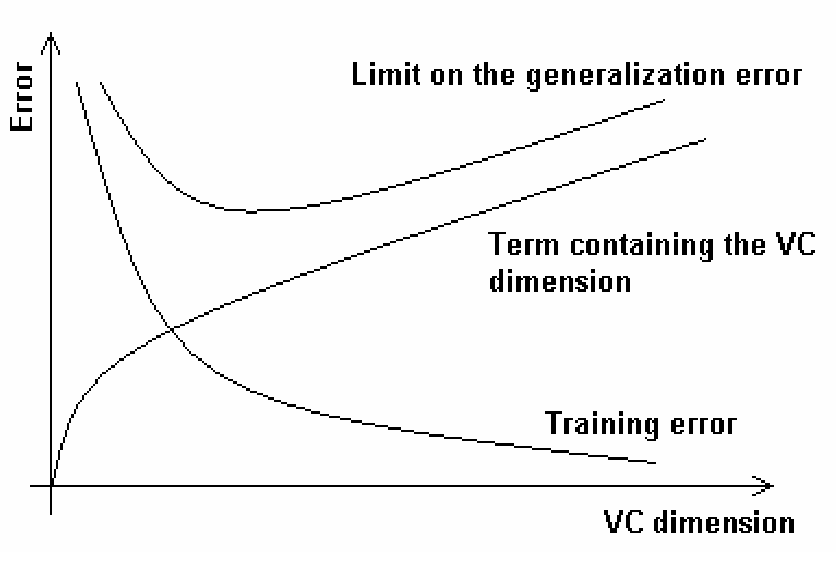
\includegraphics[width=0.5\linewidth]{img/Illustration-of-the-Structural-Risk-Minimization-Principle.png}
\end{figure}

\subsection{Validation}

Validation takes place after model training, which determines the weight parameters $w_0, w_1, \dots w_n$ to use for the $h$. The construction of a model can be divided into:

\begin{itemize}
    \item \textbf{Model selection}: estimating the generalization error of different models and choosing the best one (this includes searching for the best hyper-parameters of the model) $\xrightarrow{}$ it returns a model

    \item \textbf{Model assessment}: once a model has been chosen and both parameters and hyper-parameters have been adjusted, evaluating its generalization error on new test data as a way to measure its "quality" $\xrightarrow{}$ it returns an estimation
\end{itemize}

Among the different techniques, two simple ones are hold-out cross validation and k-fold cross validation.

With hold-out cross validation, the entire available dataset is divided into three partitions: the training set TR, the validation set VL, and the test set TS. TR is used to run the training algorithm; VL is used to select the best model; TS is used to measure the quality of the final model.

Simple hold-out cross validation can make insufficient use of data. An alternative method is called k-fold cross validation. The dataset $D$ is split into $k$ partitions, $D_1, D_2, ..., D_k$. The training algorithm uses $D/D_i$, and then the validation/test phase is done by using $D_i$. This way all the data is used for both training and validation/testing.

The main issues in using this method are choosing the value of $k$, and the fact that's pretty computationally expensive.

\paragraph{Confusion Matrix}

\begin{itemize}
    \item \textbf{Specificity}: $\dfrac{TN}{FP + TN}$

    \item \textbf{Sensitivity}: $\dfrac{TP}{TP + FN}$

    \item \textbf{Precision}: $\dfrac{TP}{TP + FP}$

    \item \textbf{Accuracy}: $\dfrac{TP + TN}{total}$
\end{itemize}

\begin{figure}[h]
    \centering
    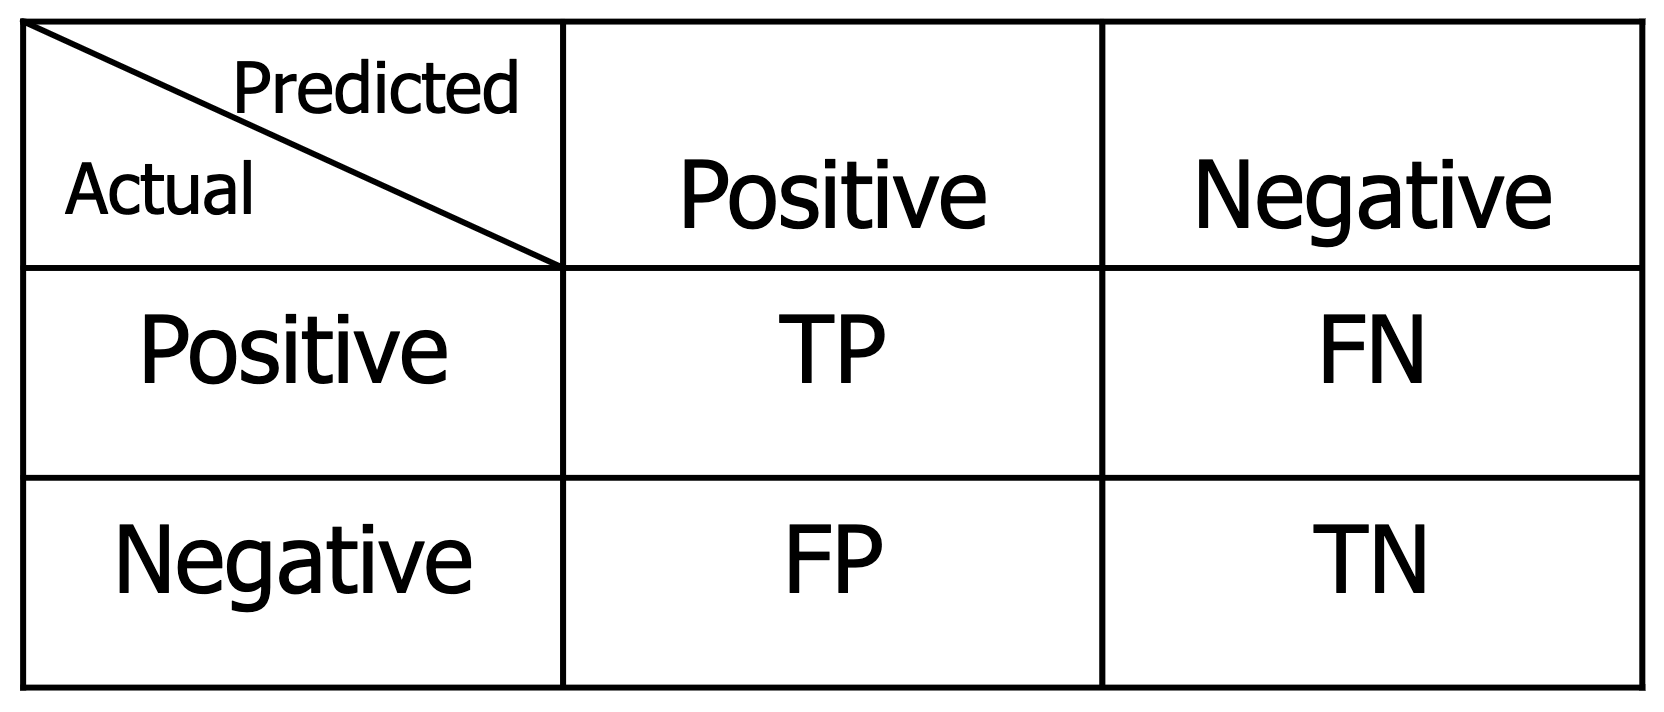
\includegraphics[width=0.5\linewidth]{img/Screenshot 2023-10-04 alle 21.11.26.png}
\end{figure}

